% !TEX root=/home/tavant/these/manuscript/src/manuscript.tex


\section{The Hall effect Thruster }
\label{sec-HET}

The \ac{HET} is an electrostatic electrical propulsion system accelerating ions by the mean of an imposed voltage difference.
\Cref{fig-bhtonoff} shows a picture of an \ac{HET} switch on and off.
We can clearly see the plasma in the annular chamber.


\begin{figure}[hbtp]
  \centering
  \includegraphics[width=\defaultwidth]{PPS-ON_OFF.jpg}
  \caption{Front view off an \ac{HET}, the BHT-1500 from Busek, USA}
  \label{fig-bhtonoff}
\end{figure}

We can summarize the composition of an \ac{HET} with four parts\string:
\begin{enumerate}
  \item The annular chamber.
  \item The injecting anode
  \item The cathode
  \item The magnetic circuit
\end{enumerate}

\begin{figure}[hbtp]
  \centering
  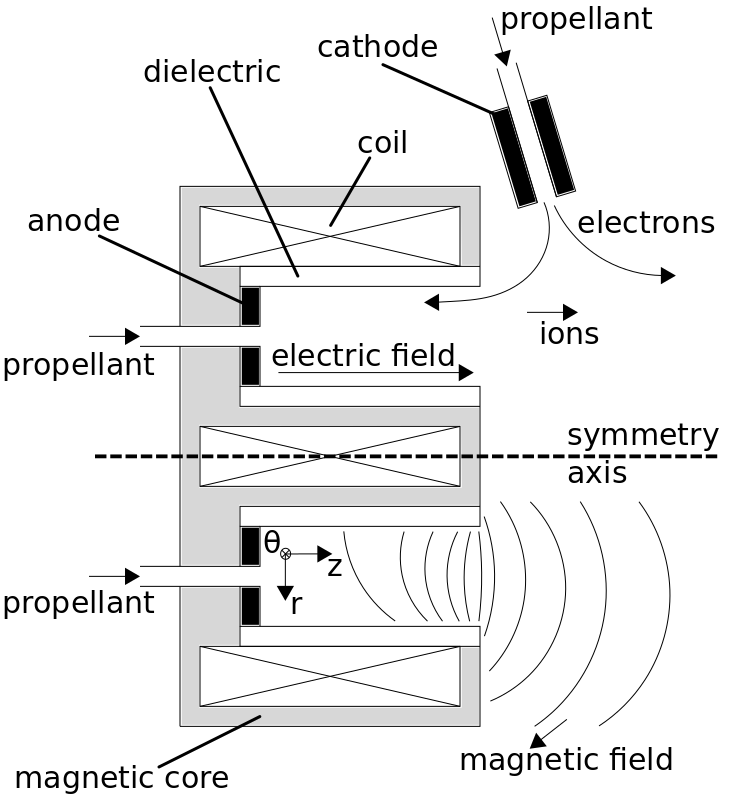
\includegraphics[width=\defaultwidth]{shematic_HET}
  \caption{Schematic cut of an \ac{HET}, illustrating its different parts. }
  \label{fig-shematiccut}
\end{figure}

\Cref{fig-shematiccut} presents a schematic cut of the \ac{HET} along its axial and radial direction.

\paragraph{The chamber} has an annular shape.
It is closed at the anode side, and kept open at the other side.
The axial length of the chamber is between $1$ and $3\,\centi\meter$, the radial width of the chamber is between $1$ and $2\,\centi\meter$. 
The walls are usually constituted by a ceramic, as the \ac{BNSiO2}.
The material needs to be resistant to erosion by ion impact sputtering.
But changing the material is also known to affects the discharge behaviour.
The usually supposed phenomena for this impact is the secondary electron emission yield that is a function of the material nature.


\paragraph{The anode} is at the bottom of the chamber.
The anode voltage is imposed to a few hundred volts.
Usually, the neutral gas injection is made by the anode itself, or it is close to the anode.
The mass flow rate is of the order of a flew mg/s.

\paragraph{The cathode} is outside of the chamber.
It is grounded, and injects electrons for two reasons\string:
\begin{itemize}
  \item most of the electrons ($\sim 90 \%$) are used to neutralize the ion flux, for both allowing the ions to leave the thruster and avoid charging of the spacecraft.
  \item some of the electrons are attracted by the anode, hence entering the chamber and allowing the plasma discharge to switch and remain on.
\end{itemize}

\paragraph{The magnetic circuit} is composed of electromagnets and a magnetic circuit mode of different ferromagnetic pieces.
It create a constant radial magnetic field in the annular chamber.
The maximum value of the radial magnetic field is located close to the exit plan of the chamber.
Its amplitude is on the order of $200$ Gauss ($\sn{2}{-2}$ T).

\Cref{fig-bshape} illustrate the axial profile of the amplitude of the radial magnetic field.
\begin{figure}[hbtp]
  \centering
  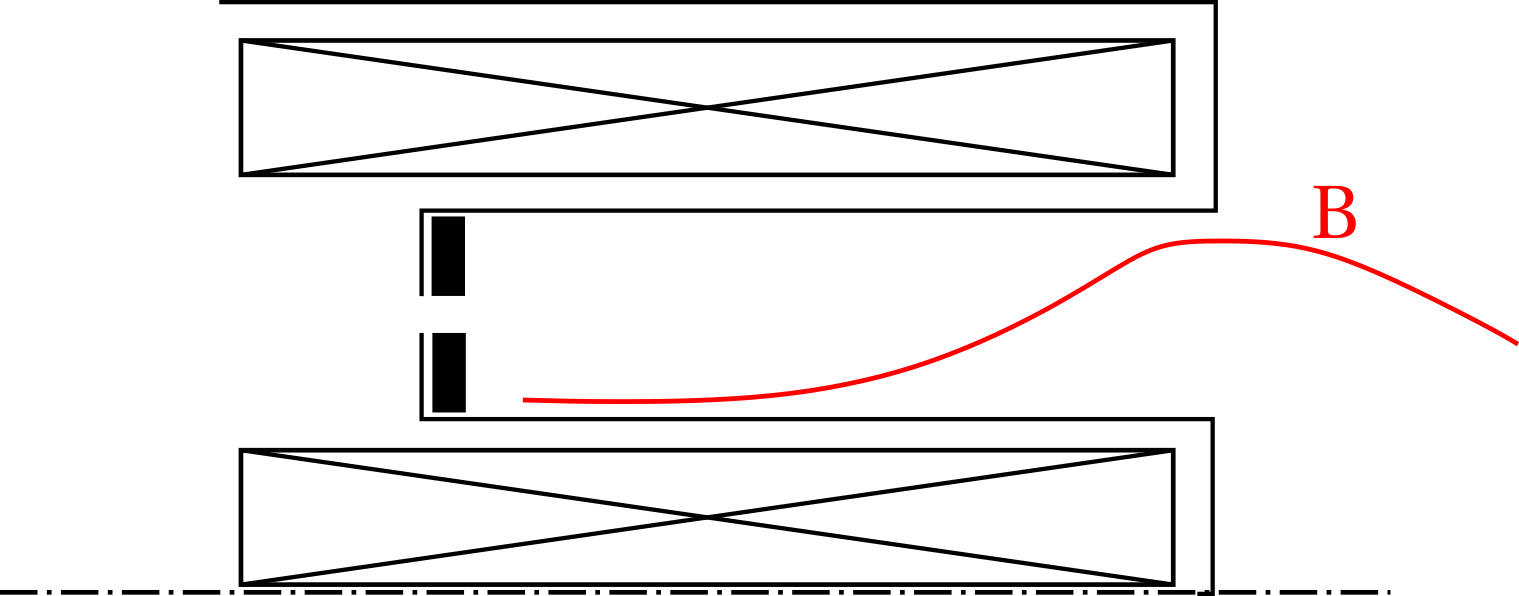
\includegraphics[width=\defaultwidth]{bshape}
  \caption{Usual shape of the axial profile of the radial magnetic field on the centreline of the channel.}
  \label{fig-bshape}
\end{figure}


\subsection{Operating principle}

The operation principle of an \ac{HET} is rather simple.
The objective is to ionize the propellant and impose an electric field to accelerate the ions.

\paragraph{Ionization}
Due to the low pressure (around $\sn{1}{-4}$ Pa), the mean free path of the electrons is larger than the chamber size.
In consequence, we impose the magnetic field in order to trap the electrons in a cyclotron motion, increasing the residence time of the electron, and the ionization.
In average, 90\% of the propellant is ionized in an well designed \ac{HET}.

\paragraph{Acceleration}
The potential difference  between the anode and the cathode is used to accelerate the ions outside of the chamber and create the thrust.
Because the magnetic field slows the electrons down, the plasma resistivity increases in the region where the magnetic field amplitude is large.
Hence, the axial profile of the amplitude of the axial electric field presents a maximum close to the maximum of the magnetic field.

\paragraph{Ionization and Acceleration regions overlay}
As both the ionization region and the acceleration region are governed by the magnetic field, it can be difficult to obtain a net separation.
However, if ionization append in the acceleration region, the newly created ions will not be accelerated at their maximum velocity, hence resulting in a loss compared to the maximum theoretical thrust.

\Cref{fig-zones} shows an illustration of the amplitude of the ionization and the acceleration due tot he electric field.
\begin{figure}[hbtp]
  \centering
  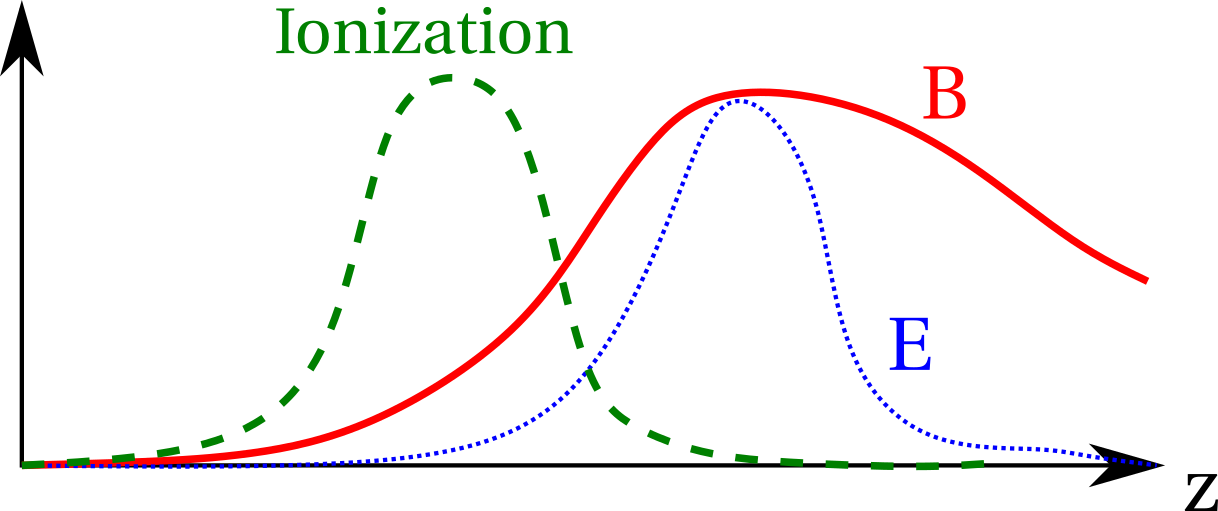
\includegraphics[width=\defaultwidth]{zones}
  \caption{Illustration of the usual axial profiles of the ionization and acceleration amplitude compared to the magnetic field.}
  \label{fig-zones}
\end{figure}

The thruster efficiency, in the usual configuration, is governed by its magnetic field topology.
Hence, it can be difficult to find the best topology that will optimize the ionization and the location of the regions.

Some concepts of double stage \ac{HET} have been proposed to decouple the two phenomena in order to control them independently.
However, the preliminary results are not as satisfactory as expected.
Moreover, the double-stage system needs more parts and power sources, resulting in a more complicated system.

\subsection{Electron drift and azimuthal instability}
The axial electric field $E$ and the radial magnetic field $B$ induces an azimuthal $E\times B$ drift of the electrons.
Because o their large mass, the ions are not significantly affected by the magnetic field, hence they do not drift.

As a consequence, they is a strong drift of the electron in respect  to the ions.
This drift can lead to instability in the azimuthal directions.
Because the drift is perpendicular to the magnetic field, it is usually called \ac{ECDI}.
However, as it rises from an $E\times B$ drift, some authors uses the name \ac{EDI}.

Azimuthal oscillations have been observed both experimentally and in simulations.
However, as the \ac{ECDI} characteristic are very close to usual \ac{IAW}, the community is still arguing about the actual kind of wave observed.
A part of the work conducted during my theses concerns the study and characterization of the instabilities observed in the simulations.

\subsection{Plasma-wall interaction}
The ceramic wall closes the chamber in the radial directions.
As usually observed in bounded plasmas, a floating plasmas sheath forms between the plasma and the dielectric wall.
The sheath confines the electrons in the plasma and accelerates the ions toward the walls.
This allows to obtain a flux of electron equals to the flux of ion, resulting in a charge conservation in the plasma, and a neutral flux, also named zero-net current to the surfaces.

Due to the relatively high electron energy, the material can emit electrons induced by electron impact.
These secondary electrons are accelerated toward the plasma, and so modify the plasma and the sheath properties.
The probability of \ac{SEE} depends of the electron impact characteristics (energy, angle) but also of the material\string: some material are more emitting than others.


\subsection{Cross field transport of the elections}
\label{sec-mob}
The electrons are not only drifting in the azimuthal directions.
For instance, because of collisions, the electrons can move from one magnetic line to another.
This leads to a cross-field transport in the direction of the electric field.
Indeed, considering the electron momentum conservation equation \citep{lafleur2016a}
\begin{equation} \label{eq-elec_momentum_mobility}
  \partial_t(m_e n_e \vect{v}_{de}) + \grad \cdot (m_e n_e  \vect{v}_{de} \vect{v}_{de}) = q_e n_e ( \vect{E} + \vect{v}_{de} \times \vect{B}) - \grad \cdot \vect{\Pi}_e - m_e \nu_m n_e \vect{v}_{de},
\end{equation}
where $m_e, q_e$, $n_e$, $\vect{v}_{de}$ and $\vect{\Pi}_e $ are the electron mass, charge, density, drift velocity and pressure tensor, and $\nu_m$ is the electron-neutral momentum transfer collision frequency.
Ignoring the electron inertia and the pressure term, and with $\vect{B} = B_0 \vect{e}_r$, we can write the balance equation projected on the axial and azimuthal direction
\begin{equation} \label{eq-elec_momentum_mobility2}
\begin{cases}
  0 =  n_e E_z - n_e v_{de{\theta}} B_0 - \frac{m_e}{q_e} \nu_m n_e v_{dez}\\
  0 =  n_e E_{\theta} -  n_e v_{dez} B_0 - \frac{m_e}{q_e} \nu_m n_e v_{de{\theta}}
\end{cases}
\end{equation}
Supposing no electric field in the azimuthal direction ($E_{\theta}=0$),  we can combine the two equations of \cref{eq-elec_momentum_mobility2} and have \citep{chen2006,meezan2001}
\begin{equation} \label{eq-mobility}
  \mobcla = \frac{n_e v_{dez}}{n_e E_z} = \frac{ \frac{\norm{q}}{m \nu_m}}{1 + \frac{\oce^2}{\nu_m}}
\end{equation}
with $\oce= \frac{\norm{q}B_0}{m}$ the cyclotron frequency.
However, it has been observed in \ac{HET} that the electron cross-field transport is higher than $\mobcla$ only due to collisions.
Recently, the \ac{ECDI} has been proposed to induce this so-called anomalous transport of the electrons.

Another phenomena that can leads to increased cross-field transport in the \ac{NWC}.
It is due to electron collisions with the wall, inducing \ac{SEE}.


\subsection{Three-dimensional physics}
\label{sec-3Dphi}

The physics of the \ac{HET} is really three dimensional\string:

\begin{itemize}
  \item The plasma is accelerated in the axial direction. The axial profile of the magnetic field is responsible for the performance of the thruster.
  \item The radial dimension is closed by the chamber walls. The walls are responsible for most of the plasma losses, both on the particle and energy balances.
  \item The electrons drifts in the azimuthal direction, leading to instabilities.
\end{itemize}

Consequently, when simulating an \ac{HET}, if one of the direction is not model, a part of the physics will be missing\string:
\begin{itemize}
  \item Missing axial direction\string: the ionization or the acceleration and the convection are missing
  \item Missing radial direction\string: the wall losses and interactions are missing
  \item Missing azimuthal direction\string: the \ac{ECDI} is missing, hence the electron cross-field transport is not well represented.
\end{itemize}

While \ac{3D}-simulations have recently been proposed, they uses scaling laws to simulate the system in a reasonable amount of time.
A \ac{3D} simulation at scale {1\string:1} is not yet accessible.
Hence, we need to rely on \ac{1D} or \ac{2D} simulations.
Consequently, we need to take into account the missing physics or include a model of its effects on the system.
